\chapter{Introduction to File Systems}
\paragraph{}
Computers use secondary storage devices to permanently store data. To write the
data, a computer uses one of the widely known specifications. This allows the
computer to read back the data, once written. These specifications are more
commonly known by the term File Systems. File Systems enforce a uniform method
of storing and retrieving the data. Further, their popular nature allows the
device to be read properly across Operating Systems. You must have come across
at least a couple of file systems, if you have used a computer. Windows use NTFS
as its file system. Linux people prefer to use ext4 or btrfs. You USB drive most
probably uses the FAT32 file system.\\

So when you copy a file to your hard disk, you are writing to the file system
right? Actually, it is a bit more complicated than that. The computer does not
simply create a file system on top of your physical device. To create a file
system, you first need an abstraction, called a partition. Partition is a
logical slice of your physical device. It acts as a container onto which a file
system can be created. The partition maps to further abstracted versions of
physical locations on the drive. Suffice to say, a partition does not
necessarily have to occuppy the whole storage device. There can be more than one
partition and each partition can have different file systems, independant from
the rest of the partitions.\\

The process of creating partitions to store data on a storage device is called
disk partitioning. Apparently, ghosts of magnetic storage media are going to
haunt us for a very long time. You can read more about disk partitioning in the
next chapter.


\chapter{Disk Partitioning}
\paragraph{}
The term disk partitioning might bring up memories of slicing a pie. But let me
assure you, disk partitioning is an entirely logical process. Disk partitioning
makes a secondary storage device usable. It creates partitions, which are then
formatted with a file system of our choice, and then used to store data. What
if you just want a single partition that spans an entire drive? You can ofcourse
do that. Still, the process you performed will be called partitioning.\\

It is very common to see systems with multiple partitions, and with a good
reason. Multiple partitions allow your system to be more flexible. There are
plethora of use cases for splitting up your disk, some of which are listed
below.


\chapter{Existing System Approach}
In existing system data reliability, data availability, and response time are dealt with data replication strategies. However, storing replicas data over a number of nodes increases the attack surface for that particular data.For example, storing m replicas of a file in a cloud instead of one replica increases the probability of a node holding file to be chosen as attack sufferer, from 1/n to m/n where n is the total number of nodes. Existing system was not achieving proper security.
\section{Disadvantages}
\begin{itemize}
	\item   A key factor determining the throughput of a cloud that stores data is the data retrieval time.
	\item   In large-scale systems, the problems of data reliability, data availability, and response time are dealt with data replication strategies.
	\item   However, placing replicas data over a number of nodes increases the attack surface for that particular data.
	\item   Affected on security and performance.  
\end{itemize}
\section{Data Fragmentation}
The security of a large-scale system, such as cloud depends on the security of the
system as a whole and the security of individual nodes. A successful intrusion into a single
node may have severe consequences, not only for data and applications on the victim node,
but also for the other nodes. The data on the victim node may be revealed fully because
of the presence of the whole le. A successful intrusion may be a result of some software or
administrative vulnerability. In case of homogenous systems, the same aw can be utilized
to target other nodes within the system. The success of an attack on the subsequent nodes
will require less effort as compared to the effort on the rst node. Comparatively, more effort
is required for heterogeneous systems. However, compromising a single le will require the
effort to penetrate only a single node. The amount of compromised data can be reduced by
making fragments of a data le and storing them on separate nodes. A successful intrusion
on a single or few nodes will only provide access to a portion of data that might not be of
any signicance. Moreover, if an attacker is uncertain about the locations of the fragments,
the probability of nding fragments on all of the nodes is very low. Consider a cloud with
M nodes and a le with z number of fragments. Let s be the number of successful intrusions
on distinct nodes,\linebreak
such that s > z
\paragraph{}
The probability that s number of victim nodes contain all of the z sites storing the le
fragments ( represented by $P(s,z)$ )is given as:

\[
P(s, z)=
\frac{
	\begin{pmatrix}
	s \\
	z 
	\end{pmatrix}
	\begin{pmatrix}
	M - s \\
	s - z
	\end{pmatrix}
}{\begin{pmatrix}
	M \\
	s
	\end{pmatrix}}
\]
\section{Centrality}
\paragraph{}
The centrality of a node in a graph provides the measure of the relative importance
of a node in the network. The node is important in the network if it:
\newline (a) interconnects more nodes than others,
\newline (b) can be reached easily by other nodes, or 
\newline(c) can reach other nodes easily.
\paragraph{}
The objective of improved retrieval time in replication makes the centrality measures
more important. There are various centrality measures; for instance, closeness centrality,
degree centrality, betweenness centrality, eccentricity centrality, and eigen- vector centrality.
Here only elaborate on the closeness, betweenness, and eccentricity centralities because here
using the aforesaid three centralities in this work.
\subsection{Betweenness Centrality} 
\paragraph{}
The betweenness centrality of a node n is the number of the shortest paths, between
other nodes, passing through n. Formally, the betweenness centrality of any node v in a
network is given as:

\[
C_{b}(\upsilon) = \sum_{ a \ \neq \  \upsilon \ \neq \ b} \frac{\delta_{ab}(\upsilon)}{\delta_{ab}}
\] 

\subsection{Closeness Centrality}
\paragraph{}
A node is said to be closer with respect to all of the other nodes within a network, if
the sum of the distances from all of the other nodes is lower than the sum of the distances
of other candidate nodes from all of the other nodes. The lower the sum of distances from
the other nodes, the more central is the node. Formally, the closeness centrality of a node
v in a network is dened as:
\linebreak
\[
C_{c}(\upsilon) = \frac{N - 1}{ \sum _{ a \neq \upsilon} d(\upsilon, a)}
\]

\paragraph{}
where N is total number of nodes in a network and d(v,a)represents the distance between
node v and node a.
\subsection{Eccentricity}
\paragraph{}
The eccentricity of a node n is the maximum distance to any node from a node n. A
node is more central in the network, if it is less eccentric. Formally, the eccentricity can be
given as:
$$ E(\upsilon_{a}) = max _{b} \ d(\upsilon_{a},\upsilon_{b}) $$
\section{T-Coloring}
\paragraph{}
Consider a graph G=(V,E)and a set T containing non-negative integers including 0.
The T- coloring is a mapping function f from the vertices of V to the set of non-negative
integers, such that f(x)- f(y) is not an element of T, where(x,y) is an element of E. The
mapping function f assigns a color to a vertex. In simple words, the distance between the
colors of the adjacent vertices must not belong to T. Formulated by Hale, the T-coloring
problem for channel assignment assigns channels to the nodes, such that the channels are
separated by a distance to avoid interference.

\chapter{Proposed System}
The proposed system called DROPS(Division and Replication of Data in Cloud for Optimal Performance and Security) jointly approaches the security and performance issues. The proposed DROPS scheme ensures that even in the case of a successful attack, no meaningful information is disclosed to the attacker. The DROPS technique doses not depend on traditional cryptographic techniques for data security. The non-cryptographic nature of the proposed scheme makes it faster to perform the required operations (placement and retrieval) on the data. It make sure a controlled replication of the file fragments,
where each of the fragments is replicated only once for the purpose of improved security.
A cloud storage security scheme jointly deals with the security and performance in terms
of retrieval time.
\section{Advantages}
\begin{itemize}
	\item  Improve security.
	\item  Improve performance. 
	\item  No information is revealed to the attacker. (If an attacker is uncertain about the locations of the fragments, the probability of finding fragments on all of the nodes is very low.)
	\item  No load on single node of cloud.
	\item  Numbers of fragments are decided according to owner’s choice.
\end{itemize}
\chapter{ DROPS System Model}
\paragraph{}
A cloud that consists of M nodes, each with its own storage capacity. Let Si represents
the name of ith node and si denotes total storage capacity of Si Communication time
between Si and Sj is the total time of all of the links within a selected path from Si to Sj
represented by c(i, j). Consider N number of file fragments such that Ok denotes k -th
fragment of a file while ok represents the size of k-th fragment. Pk denote the primary
node that stores the primary copy of Ok, replication scheme for Ok denoted by Rk is also
stored at Pk and Whenever there is an update in not as an independent document. Please
do not revise any of the current designations Ok , the updated version is sent to Pk that
broadcasts the updated version to all of the nodes in Rk. Let colSi store the value of
assigned color to Si. The colSi can have one out of two values, namely: open color and
close color. The value open color represents that the node is available for storing the file
fragment. The value close color shows that the node cannot store the file fragment The
set T is used to restrict the node selection to those nodes that are at hop-distances not
belonging to T.
\paragraph*{}
In the DROPS methodology, not to store the entire file at a single node. The DROPS
methodology fragments the file and makes use of the cloud for replication. The fragments
are distributed such that no node in a cloud holds more than single fragment, so that even
a successful attack on the node leaks no significant information.

\begin{table}
	\begin{center}
		\begin{tabular}{|c|c|} 
			\hline % draw horizontal line
			Symbols & Meanings \\
			\hline
			M & Total number of nodes in the cloud \\
			\hline
			N & Total number of fragments to be placed \\
			\hline
			{$O_k$} & k-th fragment of the file \\
			\hline
			{$o_k$} & Size of {$O_k$} \\
			\hline
			{$S^i$} & i-th node \\
			\hline
			{$s_i$} & Size of {$S^i$}  \\
			\hline
			{$cen_i$} & Centrality measure of {$S^i$} \\
			\hline
			{$col_{S^i}$} & Color assigned to {$S^i$} \\								\hline
			{$r^i_k$} & Number of reads for {$O_k$} from {$S^i$} \\		
			\hline
			{$R^i_k$} & Aggregate read cost of  {$r^i_k$} \\		
			\hline
			{$w^i_k$} & Number of writes for {$O_k$} from {$S^i$} \\
			\hline
			{$W^i_k$} & Aggregate write cost of  {$w^i_k$} \\
			\hline
			{$N N^i_k$} & Nearest neighbour of {$S^i$} holding{$O_k$} \\
			\hline
			c(i,j) & Communication cost between {$S^i$} and {$S^j$} \\
			\hline
			{$P_k$} & Primary node for {$O_k$} \\
			\hline
			{$R_k$} & Replication schema for {$O_k$} \\
			\hline
			RT & Replication Time \\
			\hline
			
		\end{tabular}
		\caption{Notations and their meanings.}
	\end{center}
\end{table}

%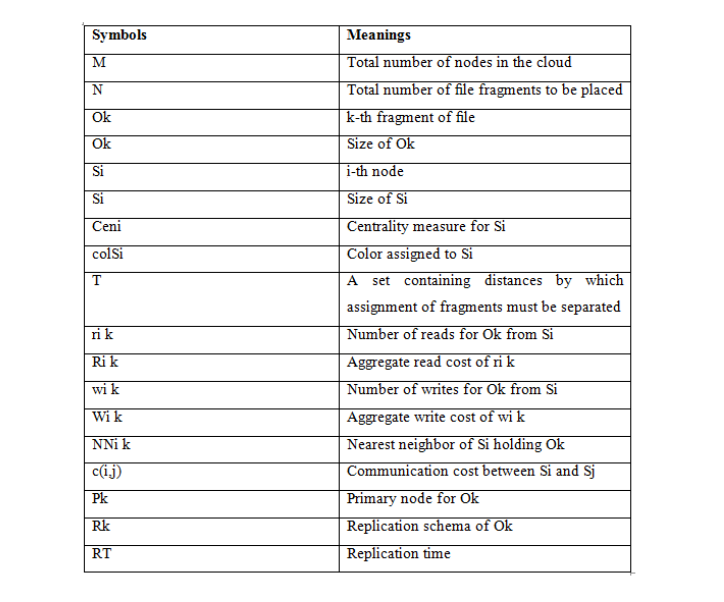
\includegraphics[scale=0.65]{meaningtable}

\paragraph*{}
\newpage
In the DROPS methodology, user sends the data file to cloud. The cloud manager
system(a user facing server in the cloud that entertains user’s requests) upon receiving the file performs:

\begin{enumerate}
	\item fragmentation
	\item first cycle of nodes selection and stores one fragment over each of the selected node and
	\item second cycle of nodes selection for fragments replication. The cloud manager keeps
	record of the fragment placement and is assumed to be a secure entity.
\end{enumerate}

\chapter{ DROPS Architecture}

This system mainly consist of 3 modules:
\begin{figure}
	\centering
	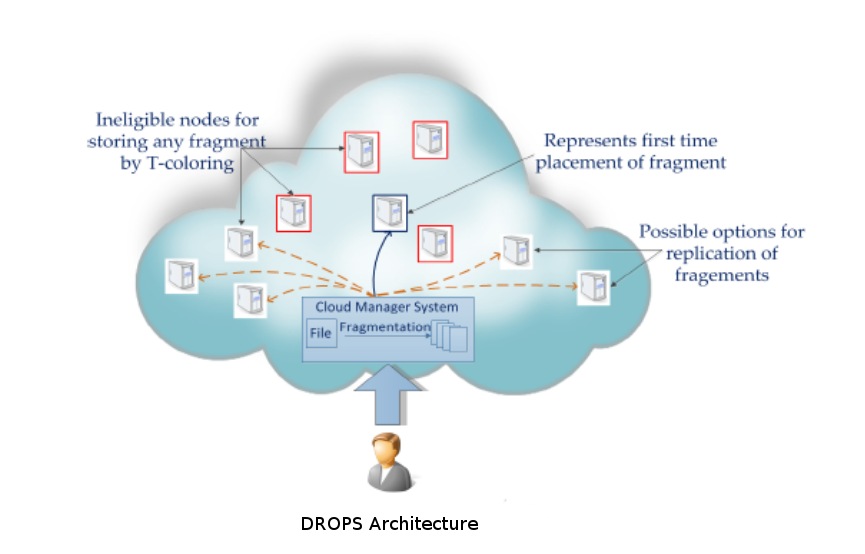
\includegraphics[width=0.95\textwidth]{./droparchitecture.png}
	\caption{DROPS Architecture}
\end{figure}
\section{Cloud Client}
\paragraph*{} 
Cloud client should be Data owner or Data user.
\subsection{Data Owner}
\paragraph*{}
Data owner is responsible for uploading file on cloud as well as view files uploaded by him or others. Data owner has information about the placed fragment and its replicas with their node numbers in cloud. 
\subsection{Data User}
\paragraph*{}
Data user is the one who is responsible for downloading files or view files uploaded by others. To download file from cloud he has to be authenticated user otherwise he will be considered as attacker.
\section{Cloud Server}
\subsection{Fragmentation}
\paragraph*{}
This approach is used for fragmenting the file for security purpose at sever side. This approach runs the Fragmentation algorithm. It has file as input and produces the file fragments as output.

\subsection{Replication}
\paragraph*{}
This approach creates replicas (duplicate copy) of fragments. These replicas are useful
when one of fragment is corrupted by attacker then to provide file for user admin replaces
its replica at that place and combine all fragments and send file to authenticated user or
data owner. To make replicas of file fragments this approach runs replication algorithm
which takes input as fragments and produces its replicas as output.

\subsection{Allocation}
\paragraph*{}
After the file is spitted and replicas are generated then allocate that fragments at
cloud server for storing data. While storing or allocating that fragments, consider security
issues. So the proposed method using T- Coloring Graph concept for placing fragments
at different nodes on cloud server. This approach runs Fragment allocation algorithm
which takes input as fragments and produces the output as fragments allocated with node
numbers.

\section{Admin}
\paragraph*{} 
Admin is an authorized person who has rights to validate authorized data owner
and user. He is also responsible for allocation of block and maintains information and
authentication.
\section{Fragment Placement}
\paragraph*{}
In the DROPS methodology, not to store the entire le at a single node. The DROPS
methodology fragments the le and makes use of the cloud for replication. The fragments
are distributed such that no node in a cloud holds more than a single fragment, so that even
a successful attack on the node leaks no signicant information. The DROPS methodology
uses controlled replication where each of the fragments is replicated only once in the cloud
to improve the security. Although, the controlled replication does not improve the retrieval
time to the level of full-scale replication, it signicantly improves the security.The fragment placement strategy is presented in
the algorithm given below.
\\
\begin{figure}
	\centering
	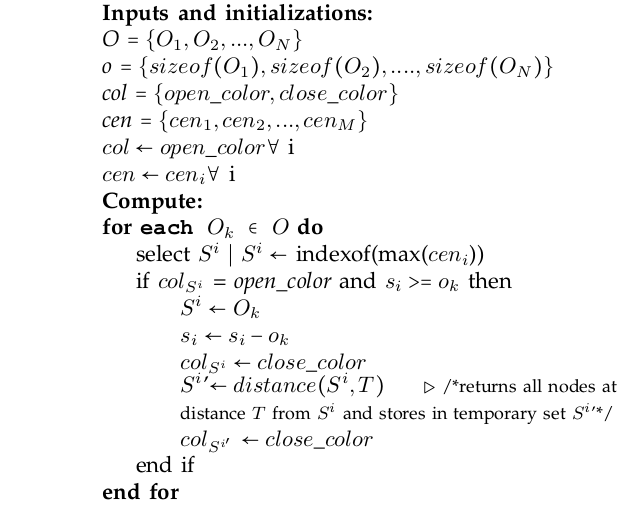
\includegraphics[scale=0.5]{placementalgo}
%	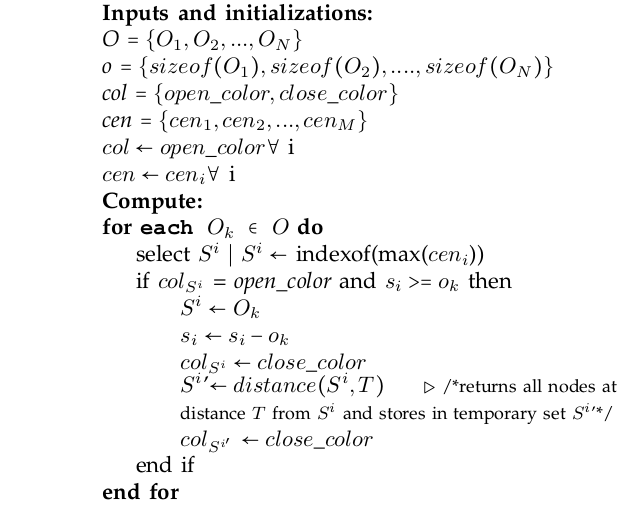
\includegraphics[width=0.9\textwidth]{./placementalgo.jpg}
	\caption{Algorithm for Fragment Placement}
\end{figure}

\paragraph*{}

Initially, all of the nodes are given the open color. Once a fragment is placed on the
node, all of the nodes within the neighborhood at a distance belonging to T are assigned
close color. In the aforesaid process, lose some of the central nodes that may increase the
retrieval time but achieve a higher security level. If somehow the intruder compromises
a node and obtains a fragment, then the location of the other fragments cannot be de-
termined. The attacker can only keep on guessing the location of the other fragments.
However,the probability of a successful coordinated attack is extremely minute. The pro-
cess is repeated until all of the fragments are placed at the nodes. The above algorithm
represents the fragment placement methodology.
\section{Fragment Replication}
\paragraph*{}
In addition to placing the fragments on the central nodes, this approach also per-
form a controlled replication to increase the data availability, reliability, and improve data
retrieval time. Place the fragment on the node that provides the decreased access cost
with an objective to improve retrieval time for accessing the fragments for reconstruction
of original le. While replicating the fragment, the separation of fragments as explained in
the placement technique through T- coloring, is also taken care off.
\paragraph*{}
In case of a large number of fragments or small number of nodes, it is also possible
that some of the fragments are left without being replicated because of the T-coloring.
As discussed previously, T-coloring prohibits to store the fragment in neighborhood of a
node storing a fragment, resulting in the elimination of a number of nodes to be used for
storage. In such a case, only for the remaining fragments, the nodes that are not holding
any fragment are selected for storage randomly. The replication strategy is presented in
the algorithm given below.
\begin{figure}
	\centering
	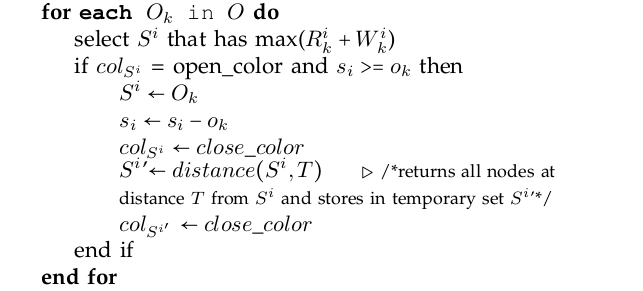
\includegraphics[scale=0.5]{replicationalgo}
	\caption{Algorithm for Fragment Replication}
\end{figure}
\section{Replication Time}
\paragraph*{}
Aim is to minimize the overall total network transfer time or replication time (RT)
or also termed as replication cost (RC). The RT is composed of two factors: (a) time due
to read requests and (b) time due to write requests.

\begin{itemize}
	\item The total read time of Ok by Si from NNi k is denoted by Ri k and is given by:
	$$ R_{k}^{i} = r_{k}^{i}o_{k}c(i , N N_{k}^{i})$$
	\item The total time due to the writing of Ok by Si ad- dressed to the Pk is represented as Wi
	k and is given:
	\[
	W_{k}^{i} = w_{k}^{i}o_{k}(c(i, P_{k})+ \sum_{ (j \in\neq R_{k}) , j \neq i} c(P_{k}, j))
	\]
	\item The overall RT is represented by:
	\[
	RT = \sum_{i = 1}^{M} \sum_{ k = 1}^{N} (R_{k}^{i} + W_{k}^{i})
	\]
	\item The storage capacity constraint states that a file fragment can only be assigned to a
	node, if storage capacity of the node is greater or equal to the size of fragment.
	\item To handle the download request from user, the cloud manager collects all the fragments from the nodes and reassemble them into a single file. Afterwards, the file is sent to the
	user.
\end{itemize}
\section{Features of DROPS}
\begin{itemize}
	\item It ensures that even in case of a successful attack, no meaningful information is revealed
	to the attacker.
	\item A successful attack on a single node must not reveal the locations of other fragments
	within the cloud.
	\item The nodes storing the fragments, are separated with certain distance by means of graph
	T-coloring to prohibit an attacker of guessing the locations of the fragments.
	\item Does not rely on the traditional cryptographic techniques for the data security.
	\item Faster
	\item Higher level of security with slight performance overhead.
\end{itemize}
